\documentclass{standalone}
\usepackage{tikz}
\usepackage{ctex,siunitx}
\usepackage{tkz-euclide}
\usepackage{amsmath}
\usetikzlibrary{patterns, calc}
\usetikzlibrary {decorations.pathmorphing, decorations.pathreplacing, decorations.shapes,}
\begin{document}
\small
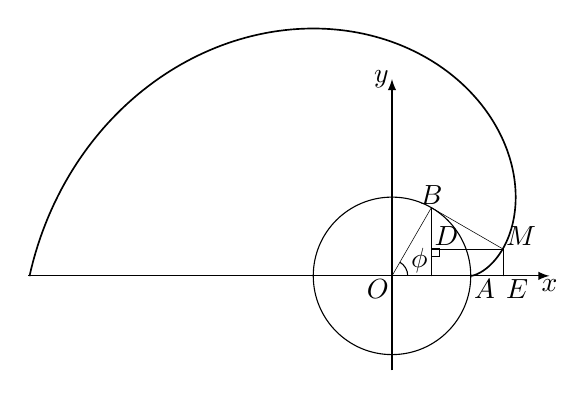
\begin{tikzpicture}[>=latex,scale=1.0,inner sep=1pt]
  \tkzDefPoints{0/0/O,1/0/A}
  \tkzDefPoint(60:1){B}
  \tkzDefPoint({0.5+pi/6*sqrt(3)},{sqrt(3)/2-pi/6}){M}
  \tkzDefPointsBy[projection=onto O--A](M,B){E,C}
  \tkzDefPointsBy[projection=onto B--C](M){D}
  \draw[thin,->](-4.62,0)--(2,0)node[below]{$x$};
  \draw[thin,->](0,-1.2)--(0,2.5)node[left]{$y$};
  \draw(0,0)circle(1);
  \draw[semithick,domain=0:257.5,samples=200] plot ({cos(\x)+\x/180*pi*sin(\x)},{sin(\x)-\x/180*pi*cos(\x)});
  \tkzDrawSegments(O,B B,M M,E B,C M,D)
  \tkzMarkAngle[size=0.2](A,O,B)
  \tkzLabelAngle[pos=0.4](A,O,B){$\phi$}
  \tkzMarkRightAngle[size=0.1](C,D,M)
  \tkzLabelPoints[below left](O)
  \tkzLabelPoints[above](B)
  \tkzLabelPoints[below right](A,E)
  \tkzLabelPoints[above right](M,D)
\end{tikzpicture}
\end{document}